\chapter{逆合成分析与多步策略}\label{ch:b2:retrosynthesis}

黑板上画着一个分子，却没有人知道如何制备它。若从架子上现有的试剂出发、顺向尝试各种反应，
则毫无头绪，因为可能性太多。化学家则反过来，从\omterm{def:b2:retrosynthesis:analysis}{目标分子}出发，朝着架子上的原料逐步回推，
在纸上每次\omterm{def:b2:retrosynthesis:disconnection}{切断}一根键，每一次\omterm{def:b2:retrosynthesis:disconnection}{切断}都相当于撤销一个已知可行的反应，
直到剩下的片段都是可以购得的化合物。本章将前几章的反应转化为这种逆向推理，
并进一步讨论如何评判由此得到的路线。

\begin{recall}
\Cref{ch:b2:alkene-redox} 至 \cref{ch:b2:wittig}：需要被逆向使用的反应。本科一年级分册：
保护基与缩醛、格氏试剂与极性反转、威廉姆森合成、
化学\omterm{def:b2:continuous-reactors:selectivity}{选择性}、醇的氧化。第 1 册：原子经济性。
\end{recall}

\section{逆向思考}

\begin{definition}[逆合成分析]\label{def:b2:retrosynthesis:analysis}
待制备的分子称为\emph{目标分子}\index{目标分子}。\emph{逆合成分析}
\index{逆合成分析}从目标分子出发，逐步回推至可获得的起始原料，
每一步都是某个已知反应的逆过程；逆合成步骤用双箭头 $\Rightarrow$ 表示，
读作“由……制得”。
\end{definition}

\begin{definition}[切断与合成子]\label{def:b2:retrosynthesis:disconnection}
\emph{切断}\index{切断}是对\omterm{def:b2:retrosynthesis:analysis}{目标分子}某根键的假想断开，
即成键反应的逆过程。异裂地切断一根键，得到两个\emph{合成子}\index{合成子}，
即理想化的带电片段：一个是给体（亲核的，通常带负电），另一个是受体（亲电的，通常带正电）。
\emph{合成等价物}\index{合成等价物}是能起到合成子作用的真实试剂：
碳负离子 \ce{R-} 对应格氏试剂，
碳正离子 $\mathrm{R\overset{+}{C}H{-}OH}$ 对应醛。
\end{definition}

\begin{definition}[官能团转换]\label{def:b2:retrosynthesis:fgi}
\emph{官能团转换}\index{官能团转换}（FGI）是一种逆合成步骤，
它改变官能团，而不改变碳骨架：
由酮还原得到醇，由烯烃加氢得到烷烃链，由酰胺得到胺。
\end{definition}

\begin{omfigure}
\begin{tikzpicture}[every node/.style={align=center}]
\node (T) at (0,0) {\setchemfig{atom sep=1.7em}\chemfig{Ph-CH(-[2]OH)-CH(-[6]CH_3)-CH_3}};
\node (A) at (-4.6,-2.6) {\ce{PhCHO}\\[1pt] + \ce{(CH3)2CHMgBr}};
\node (B) at (0,-2.6) {\ce{PhMgBr}\\[1pt] + \ce{(CH3)2CHCHO}};
\node (C) at (4.6,-2.6) {\setchemfig{atom sep=1.7em}\chemfig{Ph-C(=[2]O)-CH(-[6]CH_3)-CH_3}};
\node (D) at (4.6,-5.0) {\ce{C6H6}\\[1pt] + \ce{(CH3)2CHCOCl}};
\draw[omretro] (T.south west) -- node[above left, font=\small] {a} (A.north);
\draw[omretro] (T.south) -- node[right, font=\small] {b} (B.north);
\draw[omretro] (T.south east) -- node[above right, font=\small] {FGI} (C.north);
\draw[omretro] (C.south) -- node[right, font=\small] {c} (D.north);
\end{tikzpicture}
\par\vspace{6pt}

{\small 2-甲基-1-苯基丙-1-醇的逆合成树。(a) 与 (b)：醇碳旁边 \ce{C-C} 键的两种\omterm{def:b2:retrosynthesis:disconnection}{切断}，
各得一个醛和一个格氏试剂。FGI：由酮还原得到醇；
(c) 由苯经\omterm{def:b2:aromatic-substitution:friedel-crafts}{傅–克酰基化}得到酮。
每个箭头均读作“由……制得”。}
\end{omfigure}

树状图体现了该方法的几个习惯。\omterm{def:b2:retrosynthesis:disconnection}{切断}总是选在官能团旁边的键上，
因为反应正是在那里成键的。每一次\omterm{def:b2:retrosynthesis:disconnection}{切断}都要写出\omterm{def:b2:retrosynthesis:disconnection}{合成子}，并为之找到真实试剂加以核对。
而且答案很少只有一个：这棵树会分叉，
各分支最终在\cref{sec:b2:retrosynthesis:judging}中加以评判。

\begin{omfigure}
\begin{center}
\small
\renewcommand{\arraystretch}{1.25}
\begin{tabular}{lll}
\hline
\omterm{def:b2:retrosynthesis:disconnection}{合成子} & 类型 & \omterm{def:b2:retrosynthesis:disconnection}{合成等价物} \\
\hline
\ce{R-}（烷基、芳基） & 给体 & \ce{RMgBr}、\ce{RLi}、\ce{R2CuLi}（\omterm{def:b2:conjugate-additions:addition-modes}{共轭加成}） \\
$\mathrm{^-CH_2COR}$ & 给体 & \ce{CH3COR} 的\omterm{def:b2:enolates-aldol:enolate}{烯醇负离子}，或 3-氧代丁酸乙酯 \\
$\mathrm{^-C{\equiv}N}$ & 给体 & \ce{NaCN} \\
$\mathrm{R\overset{+}{C}H{-}OH}$ & 受体 & 醛 \ce{RCHO} \\
$\mathrm{R\overset{+}{C}{=}O}$ & 受体 & \omterm{def:b2:acyl-substitution:derivative}{酰氯} \ce{RCOCl}、酯 \\
\ce{R+}（伯） & 受体 & 卤代烃 \ce{RBr}（双分子取代） \\
$\mathrm{^+CH_2CH_2COR}$ & 受体 & 烯酮 \ce{CH2=CHCOR}（\omterm{def:b2:conjugate-additions:addition-modes}{共轭加成}） \\
\hline
\end{tabular}
\end{center}

{\small 常见\omterm{def:b2:retrosynthesis:disconnection}{合成子}及其\omterm{def:b2:retrosynthesis:disconnection}{合成等价物}。给体\omterm{def:b2:retrosynthesis:disconnection}{合成子}为碳负离子，
受体\omterm{def:b2:retrosynthesis:disconnection}{合成子}为碳正离子；真实试剂的极性相同，但不带完整电荷。}
\end{omfigure}

\section{单官能团切断}

单官能团\omterm{def:b2:retrosynthesis:disconnection}{切断}是\omterm{def:b2:retrosynthesis:disconnection}{切断}与单个官能团相邻的键。对于醚、酯或胺中的 \ce{C-O} 键或 \ce{C-N} 键，
\omterm{def:b2:retrosynthesis:disconnection}{切断}发生在碳与杂原子之间，杂原子为给体，
碳为受体（对应威廉姆森合成、\omterm{def:b2:acyl-substitution:esterification}{酯化}、酰胺的生成）。
对于 \ce{C-C} 键，官能团决定\omterm{def:b2:retrosynthesis:disconnection}{合成子}的极性：与醇碳相邻时，
醇碳为受体（得到醛或酮），另一侧的碳为给体（有机金属试剂）；
羰基旁边，$\alpha$ 碳为给体（\omterm{def:b2:enolates-aldol:enolate}{烯醇负离子}）。

多数这类反应需要在正确的位置上具有正确的氧化级别，因此各氧化级别之间的\omterm{def:b2:retrosynthesis:fgi}{官能团转换}
是路线中最常见的步骤：烯烃、醇、醛或酮、酸。其中一个问题在本科一年级分册中未能解决，
即如何使伯醇的氧化停留在醛的阶段。

\begin{proposition}[温和氧化]\label{prop:b2:retrosynthesis:mild-oxidation}
伯醇在无水有机溶剂中被氧化为醛，而不进一步氧化为酸，所用的氧化剂可以是
二氯甲烷中的氯铬酸吡啶盐，
斯文氧化（先以草\omterm{def:b2:acyl-substitution:derivative}{酰氯}活化二甲亚砜，再加入三乙胺，于低温下进行），或戴斯–马丁高碘烷。
在水中，铬（VI）或高锰酸盐则将其氧化为羧酸。
\end{proposition}

\begin{proof}[论证]
这些氧化剂夺去 \ce{C-H} 键中的氢，该氢所在的碳上连有 \ce{OH}。生成的醛
不再含有这样的基团。然而在水中，醛与其水合物 \ce{RCH(OH)2} 处于平衡，
而该水合物在带氢的碳上又连有 \ce{OH}，因此会像醇一样被氧化为酸。
若无水，则不生成水合物，氧化便
停留在醛的阶段。
\end{proof}

\section{双官能团切断}

若\omterm{def:b2:retrosynthesis:analysis}{目标分子}含有两个官能团，最好的\omterm{def:b2:retrosynthesis:disconnection}{切断}通常同时利用两者：所\omterm{def:b2:retrosynthesis:disconnection}{切断}的键
使其中一个官能团指定供体，另一个指定受体。两个官能团之间的距离，
以两个官能化碳之间的碳原子数（含两端）计，决定应采用何种反应。

\begin{proposition}[模式及其反应]\label{prop:b2:retrosynthesis:patterns}
两个官能团之间的关系与前几章的反应对应如下。
奇数关系（1,3 和 1,5）符合羰基化学的天然极性；偶数关系（1,4
和 1,6）则不然，需要极性反转，或断开一个环。
\end{proposition}


\begin{proof}[论证]
在羰基化学中，羰基碳为受体，$\alpha$ 碳为供体，烯酮
在其 $\beta$ 碳上加成一个受体。\omterm{def:b2:enolates-aldol:enolate}{烯醇负离子}（$\alpha$ 位为供体）作用于羰基（
羰基碳为受体）时，使 1、2 号碳原子成键，形成 1,3 模式：\omterm{def:b2:enolates-aldol:aldol}{羟醛}反应与\omterm{def:b2:enolates-aldol:claisen}{克莱森缩合}。\omterm{def:b2:enolates-aldol:enolate}{烯醇负离子}作用于烯酮的 $\beta$
碳上时，构成 1,5 模式：\omterm{def:b2:conjugate-additions:michael}{迈克尔加成}，再接\omterm{def:b2:conjugate-additions:robinson}{罗宾逊成环}。对于 1,4 模式，\omterm{def:b2:retrosynthesis:disconnection}{切断}后留下的
$\alpha$ 碳作为受体；普通羰基试剂都不提供这种极性，而 $\alpha$-溴代
酮却能提供，因为溴在该碳上是离去基团。1,6-二羰基化合物可由环己烯经\omterm{def:b2:alkene-redox:cleavage}{臭氧解}开环得到（见
\cref{prop:b2:alkene-redox:ozonolysis}），而环己烯由\omterm{def:b2:frontier-orbitals:diels-alder}{第尔斯–阿尔德
反应}制得（见\cref{def:b2:frontier-orbitals:diels-alder}）。
\end{proof}

\begin{omfigure}
\begin{center}
\small
\renewcommand{\arraystretch}{1.25}
\begin{tabular}{lll}
\hline
\omterm{def:b2:retrosynthesis:analysis}{目标分子}中的模式 & \omterm{def:b2:retrosynthesis:disconnection}{切断}方式 & 反应 \\
\hline
$\beta$-羟基羰基化合物（1,3） & $\alpha$--$\beta$ 键 & \omterm{def:b2:enolates-aldol:aldol}{羟醛加成} \\
$\alpha,\beta$-不饱和羰基化合物 & \ce{C=C} & \omterm{def:b2:enolates-aldol:aldol}{羟醛缩合} \\
1,3-二羰基化合物 & C(O)--C$\alpha$ & \omterm{def:b2:enolates-aldol:claisen}{克莱森缩合} \\
1,5-二羰基化合物 & 受体的 C$\alpha$--C$\beta$ & \omterm{def:b2:conjugate-additions:michael}{迈克尔加成} \\
环己-2-烯-1-酮 & 环内 \ce{C=C}，其后为迈克尔键 & \omterm{def:b2:conjugate-additions:robinson}{罗宾逊成环} \\
环己烯 & 两个环内 \ce{C-C} 键 & \omterm{def:b2:frontier-orbitals:diels-alder}{第尔斯–阿尔德反应} \\
在指定位置的烯烃 & \ce{C=C} & \omterm{def:b2:wittig:wittig}{维蒂希反应}或 HWE 反应 \\
1,4-二羰基化合物 & 中间的 \ce{C-C} & \omterm{def:b2:enolates-aldol:enolate}{烯醇负离子} + $\alpha$-卤代酮 \\
1,6-二羰基化合物 & 重新连接两端 & 环己烯的\omterm{def:b2:alkene-redox:cleavage}{氧化裂解} \\
\hline
\end{tabular}
\end{center}

{\small 双官能团\omterm{def:b2:retrosynthesis:disconnection}{切断}。前六种采用正常极性：\omterm{def:b2:enolates-aldol:enolate}{烯醇负离子}（供体）位于
羰基或烯酮（受体）上。1,4 模式需要与羰基相连的 $\alpha$ 碳充当受体，
这与其通常角色相反，而 $\alpha$-卤代酮可提供这一极性。}
\end{omfigure}

\begin{method}[逆合成分析]\label{met:b2:retrosynthesis:retrosynthesis}
\begin{enumerate}
  \item 列出\omterm{def:b2:retrosynthesis:analysis}{目标分子}的官能团及其相互关系（1,2；1,3；\dots）。
  \item 考虑\omterm{def:b2:retrosynthesis:fgi}{官能团转换}（FGI），以得到良好\omterm{def:b2:retrosynthesis:disconnection}{切断}的模式（如由酮得醇，
        由烯烃得烷烃链）。
  \item 选择关键的键：靠近官能团，位于分子中部，处于分支点，或连接环与链，
        以使各片段大小相近。
  \item 写出\omterm{def:b2:retrosynthesis:disconnection}{合成子}及其\omterm{def:b2:retrosynthesis:disconnection}{合成等价物}；舍去没有实际试剂与之对应的\omterm{def:b2:retrosynthesis:disconnection}{切断}。
  \item 检查化学\omterm{def:b2:continuous-reactors:selectivity}{选择性}：每种试剂还会与哪些其他官能团反应？需规划保护，
        或调整步骤顺序。
  \item 对每个片段重复上述过程，直至所有片段都可得到；然后按正向写出路线，注明试剂与
        反应条件。
\end{enumerate}
\end{method}

\section{路线中的保护基}

合成路线中常需要一种试剂，它会进攻分子中的第二个官能团。本科一年级分册
已将醛和酮保护为缩醛。路线可在若干保护基中选择，每种保护基
均有其专用的脱除条件：缩醛（以水溶液中的酸脱除），醇的硅醚（以
氟离子脱除），苄醚（经钯催化氢解脱除），胺的氨基甲酸酯，例如
叔丁氧羰基（以酸脱除），以及酯（以碱脱除）。

\begin{definition}[正交保护]\label{def:b2:retrosynthesis:orthogonal}
一组\emph{正交保护基}\index{正交保护基}是指这样一组保护基：
其中每一个都可在使其余各个保持完好的条件下脱除，从而可以
以任意次序逐一释放它们所掩蔽的官能团。
\end{definition}

\begin{method}[路线中的保护]\label{met:b2:retrosynthesis:protect-in-route}
\begin{enumerate}
  \item 对每一步，列出该试剂除目标基团外还会进攻的其他基团。
  \item 首先尽量避免保护：调换步骤顺序，或使用\omterm{def:b2:continuous-reactors:selectivity}{选择性}更高的试剂
        （对于酯旁的酮，宜用\omterm{def:b2:alkene-redox:hydroboration}{硼氢化}物而非氢化物）。
  \item 否则，选用在脱除前各步中均稳定、且可在分子能耐受的条件下
        脱除的保护基。
  \item 若需分别释放若干个基团，则选用一组\omterm{def:b2:retrosynthesis:orthogonal}{正交保护基}。
  \item 寻找一个可顺带脱除保护基的步骤：原本就要进行的氢化反应也会脱去
        苄醚。
  \item 核算：每次保护要多两步反应，须计入这两步的产率。
\end{enumerate}
\end{method}

\section{路线的评价}\label{sec:b2:retrosynthesis:judging}

\begin{proposition}[总产率]\label{prop:b2:retrosynthesis:overall-yield}
线性步骤序列的总产率等于各步产率之积：
$\rho = \rho_1 \rho_2 \cdots \rho_n$。若 $n$ 步的产率均为 $\rho_1$，则 $\rho = \rho_1^{\,n}$。
\end{proposition}

\begin{proof}
第 $k$ 步将其起始原料的物质的量 $n_{k-1}$ 转化为 $n_k = \rho_k\, n_{k-1}$ 的产物
（产率以中间体的物质的量计，其余试剂均足量）。由归纳法可得，
$n_n = \rho_n \rho_{n-1} \cdots \rho_1\, n_0$，于是总产率 $n_n/n_0$ 即为该乘积。
\end{proof}

\begin{omfigure}
\begin{tikzpicture}
\begin{axis}[width=0.75\linewidth, height=5.4cm, xmin=0, xmax=20, ymin=0, ymax=100,
  xlabel={步数 $n$}, ylabel={总产率（\%）}, label style={font=\small},
  tick label style={font=\scriptsize}, xtick={0,5,10,15,20}, grid=major, grid style={black!12},
  legend style={font=\scriptsize, at={(0.98,0.98)}, anchor=north east}, legend cell align=left]
\addplot[omDef, thick] table[x=n, y=r95] {figdata/out/bachelor-2-overall-yield.dat};
\addplot[omThm, thick] table[x=n, y=r90] {figdata/out/bachelor-2-overall-yield.dat};
\addplot[omMeth, thick] table[x=n, y=r80] {figdata/out/bachelor-2-overall-yield.dat};
\addplot[black!60, thick, dashed] table[x=n, y=r70] {figdata/out/bachelor-2-overall-yield.dat};
\legend{每步 95~\%, 每步 90~\%, 每步 80~\%, 每步 70~\%}
\end{axis}
\end{tikzpicture}
\par\vspace{4pt}

{\small 线性路线的总产率与其步数的关系，对应四种每步产率
（见\cref{prop:b2:retrosynthesis:overall-yield}）。每步 90~\% 时，十步后保留 35~\% 的物料；每步 70~\% 时，
十步后不足 3~\%。}
% figdata: bachelor-2/overall-yield.py
\end{omfigure}

乘积法则解释了为何短路线更占优，为何保护（需额外两步）从来不是免费的，以及为何
化学家更倾向于分别构建两半、最后再连接：长路线由此分为两条较短的支路，
一条支路的损失不会与另一条支路的损失相乘。除产率与长度外，
路线还需从\omterm{def:b2:continuous-reactors:selectivity}{选择性}（每步都应只得到一种产物）、试剂的成本
与危害，所产生的废弃物（每步的原子经济性与纯化所用的溶剂），
以及每步放大的难易程度来评判。

\begin{history}[逆向推导，明确化]
\begin{minipage}[t]{0.2\linewidth}
\vspace{0pt}
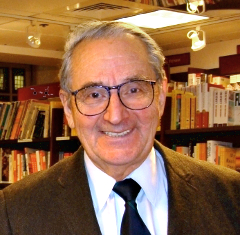
\includegraphics[width=\linewidth]{images/book3/corey.jpg}
\end{minipage}\hfill
\begin{minipage}[t]{0.76\linewidth}
\vspace{0pt}
化学家向来从目标出发逆向推理，但自 1960 年代起，埃利亚斯·詹姆斯·科里
将这一习惯化为明确的规则：\omterm{def:b2:retrosynthesis:disconnection}{切断}、\omterm{def:b2:retrosynthesis:disconnection}{合成子}、逆合成箭头，以及
甚至是应用这些规则的计算机程序。他于 1990 年获得诺贝尔化学奖，表彰其
在有机合成理论与方法上的贡献。（照片：Trvthchem 摄，CC0，维基共享资源。）
\end{minipage}
\end{history}

\begin{safety}{\ghs[5mm]{GHS02}\,\ghs[5mm]{GHS03}\,\ghs[5mm]{GHS05}\,\ghs[5mm]{GHS06}\,\ghs[5mm]{GHS07}\,\ghs[5mm]{GHS08}}
草\omterm{def:b2:acyl-substitution:derivative}{酰氯}具有腐蚀性和毒性，遇水反应放出氯化氢；
斯文氧化放出一氧化碳与有恶臭的二甲基硫醚，因此须在通风橱中进行。
戴斯–马丁高碘烷是一种氧化剂，不得加热。六价铬试剂
在有替代方法时已被尽量避免。
% ledger: ghs:oxalyl-chloride, ghs:DMSO, ghs:DMP
\end{safety}

\section{练习}

\begin{exercise}[$\star$]\label{exo:b2:retrosynthesis:1}
将每种醇\omterm{def:b2:retrosynthesis:disconnection}{切断}为一个羰基化合物和一种格氏试剂（列出所有可能）：
2-苯基丙-2-醇、戊-3-醇、1-环己基乙醇、2-甲基丁-2-醇、1-苯基乙醇。
\end{exercise}

\begin{exercise}[$\star$]\label{exo:b2:retrosynthesis:2}
对 1-苯基乙醇在 \ce{C-C} 键处的\omterm{def:b2:retrosynthesis:disconnection}{切断}，命名两个\omterm{def:b2:retrosynthesis:disconnection}{合成子}，并指出哪一个是
施主，再为每个\omterm{def:b2:retrosynthesis:disconnection}{合成子}给出\omterm{def:b2:retrosynthesis:disconnection}{合成等价物}。
\end{exercise}

\begin{exercise}[$\star$]\label{exo:b2:retrosynthesis:3}
某五步路线的各步产率分别为 90、85、80、95 和 70~\%。计算其总产率。
\end{exercise}

\begin{exercise}[$\star$]\label{exo:b2:retrosynthesis:4}
将 4-氧代戊酸乙酯转化为 5-羟基戊-2-酮。请设计带有保护
基的路线，并说明为何需要保护基。
\end{exercise}

\begin{exercise}[$\star\star$]\label{exo:b2:retrosynthesis:5}
以不超过两个碳原子的化合物为原料，提出丁-1,3-二醇的逆合成方案，
其中包括一步\omterm{def:b2:retrosynthesis:fgi}{官能团转换}（FGI）和一次双基团\omterm{def:b2:retrosynthesis:disconnection}{切断}。
\end{exercise}

\begin{exercise}[$\star\star$]\label{exo:b2:retrosynthesis:6}
\omterm{def:b2:frontier-orbitals:diels-alder}{第尔斯–阿尔德反应}可用于对 1-（环己-3-烯-1-基）乙-1-酮进行\omterm{def:b2:retrosynthesis:disconnection}{切断}。
\end{exercise}

\begin{exercise}[$\star\star$]\label{exo:b2:retrosynthesis:7}
通过\omterm{def:b2:conjugate-additions:robinson}{罗宾逊成环}对 4,4-二甲基环己-2-烯-1-酮进行\omterm{def:b2:retrosynthesis:disconnection}{切断}。
\end{exercise}

\begin{exercise}[$\star\star$]\label{exo:b2:retrosynthesis:8}
1-苯基丁-1-酮可由\omterm{def:b2:aromatic-substitution:friedel-crafts}{傅–克酰基化}一步制得，也可由苯甲醛两步制得。
写出两条路线并加以比较。
\end{exercise}

\begin{exercise}[$\star\star$]\label{exo:b2:retrosynthesis:9}
欲由己-1-醇制得己醛。哪些试剂可以得到己醛，哪一种会得到
己酸？请说明理由。
\end{exercise}

\begin{exercise}[$\star\star\star$]\label{exo:b2:retrosynthesis:10}
在 4-氨基丁-1-醇中，胺须先与\omterm{def:b2:acyl-substitution:derivative}{酰氯}在一步中反应，而醇须
随后与另一种试剂反应。请提出一对\omterm{def:b2:retrosynthesis:orthogonal}{正交保护基}及其反应顺序。
\end{exercise}

\begin{exercise}[$\star\star\star$]\label{exo:b2:retrosynthesis:11}
以 3-氧代丁酸乙酯为原料，提出己烷-2,5-二酮的合成方案，该化合物为 1,4-二羰基化合物。
\end{exercise}

\begin{exercise}[$\star\star\star$]\label{exo:b2:retrosynthesis:12}
6-甲基庚-5-烯-2-酮，\ce{(CH3)2C=CHCH2CH2COCH3}，是一种香料中间体。请以
3-氧代丁酸乙酯与一种卤代烃为原料，提出完整方案：\omterm{def:b2:retrosynthesis:analysis}{逆合成分析}、正向路线，
以及去除酯基的那一步。
\end{exercise}

\section{问题：覆盆子酮}

\begin{problem}[{周末问题——香料化合物的逆合成，酚及其是否需要保护，
钯的替代方案，以及对各路线的判断}]
\label{pb:b2:retrosynthesis:1}
覆盆子酮，即 4-（4-羟基苯基）丁-2-酮，存在于覆盆子及其他水果中，
并用作香料添加剂和香水原料。练习数据：\omterm{def:b2:enolates-aldol:aldol}{羟醛}路线的各步产率分别为 85~\%（缩合）
和 92~\%（氢化）。摩尔质量（\unit{g/mol}）：C 12.011，H 1.008，O 15.999，N 14.007，
I 126.90。酚的 $\mathrm pK_a$ 为 9.99。
% ledger: use:raspberry-ketone, aw:C, aw:H, aw:O, aw:N, aw:I, pka:phenol, ghs:raspberry-ketone, ghs:4-iodophenol, ghs:MVK

\medskip
\noindent\textbf{第一部分——\omterm{def:b2:retrosynthesis:analysis}{逆合成分析}。}
\begin{enumerate}
  \item 画出\omterm{def:b2:retrosynthesis:analysis}{目标分子}并命名其官能团。
  \item 哪一步\omterm{def:b2:retrosynthesis:fgi}{官能团转换}（FGI）可将 \ce{ArCH2CH2CO} 结构单元转化为已知\omterm{def:b2:retrosynthesis:disconnection}{切断}模式？
  \item 写出所得的不饱和酮，并标明其几何构型。
  \item 该化合物含有哪一种双基团模式？由何种反应生成？
  \item 命名两种起始原料。
  \item 为何这一交叉\omterm{def:b2:enolates-aldol:aldol}{羟醛}反应只得到一种主要产物？
  \item 写出两步正向路线，并注明反应条件。
\end{enumerate}

\medskip
\noindent\textbf{第二部分——酚。}
\begin{enumerate}[resume]
  \item 在氢氧化钠水溶液中，4-羟基苯甲醛以何种形式存在？请利用
        $\mathrm pK_a$ 进行判断。
  \item 该形式如何改变醛的亲电性？
  \item 若将酚羟基保护，则第二步会直接脱去哪一个基团？请说明理由。
  \item 计算采用该保护方案后路线的步骤数。
  \item 氢化过程中，苯环是否有被还原的风险？
  \item 是否需要保护？请给出结论。
\end{enumerate}

\medskip
\noindent\textbf{第三部分——钯催化的替代方案。}
\begin{enumerate}[resume]
  \item 在环与链之间的键处对不饱和酮进行\omterm{def:b2:retrosynthesis:disconnection}{切断}：应得到哪两种赫克
        反应底物？
  \item 写出以三乙胺为碱的赫克反应。
  \item 芳基会连接到丁-3-烯-2-酮的哪一个碳原子上？为什么？
  \item 写出\omterm{def:b2:catalytic-cycles:cycle}{催化循环}各步骤的名称。
  \item 计算赫克步骤的原子经济性（计入三乙胺）。
  \item 计算\omterm{def:b2:enolates-aldol:aldol}{羟醛缩合}的原子经济性。
\end{enumerate}

\medskip
\noindent\textbf{第四部分——评价两条路线。}
\begin{enumerate}[resume]
  \item 氢化步骤的原子经济性是多少？
  \item 计算\omterm{def:b2:enolates-aldol:aldol}{羟醛}路线的总原子经济性。
  \item 氢化还原的是哪一个双键？为什么酮基能保留？
  \item 比较两条路线所用试剂的成本与危害。
  \item 你会选择哪一条路线？
  \item 若增加一步产率为 90~\% 的反应，总产率会受到怎样的影响？
  \item 给出两步\omterm{def:b2:enolates-aldol:aldol}{羟醛}路线的总产率。
\end{enumerate}
\end{problem}
